\section{Summary of results and price-performance}\label{resultsSummary}

In this section we summarize the results obtained using the different configurations presented previously. We discuss the total execution times and monetary costs. Additionally, we introduce an adapted version of the TPC-DS metric to facilitate performance comparisons, which enables us to derive price-performance criteria. Finally, we estimate the cost effects of opting for spot EC2 instances instead of on-demand instances.

\subsection{Total execution times}\label{resultsSummaryTotalExecutionTimes}

Figure \ref{fig:resultsSummaryTotalTimes} presents the total time required for executing the TPC-DS Benchmark at the 1 TB scale factor for the different configurations that we have covered. The total times are composed from the Data Loading Test, the Power Test, and the Throughput Test times. By far the largest component is the Throughput Test in all cases.

\begin{figure}
   \begin{center}
   \scalebox{0.75}{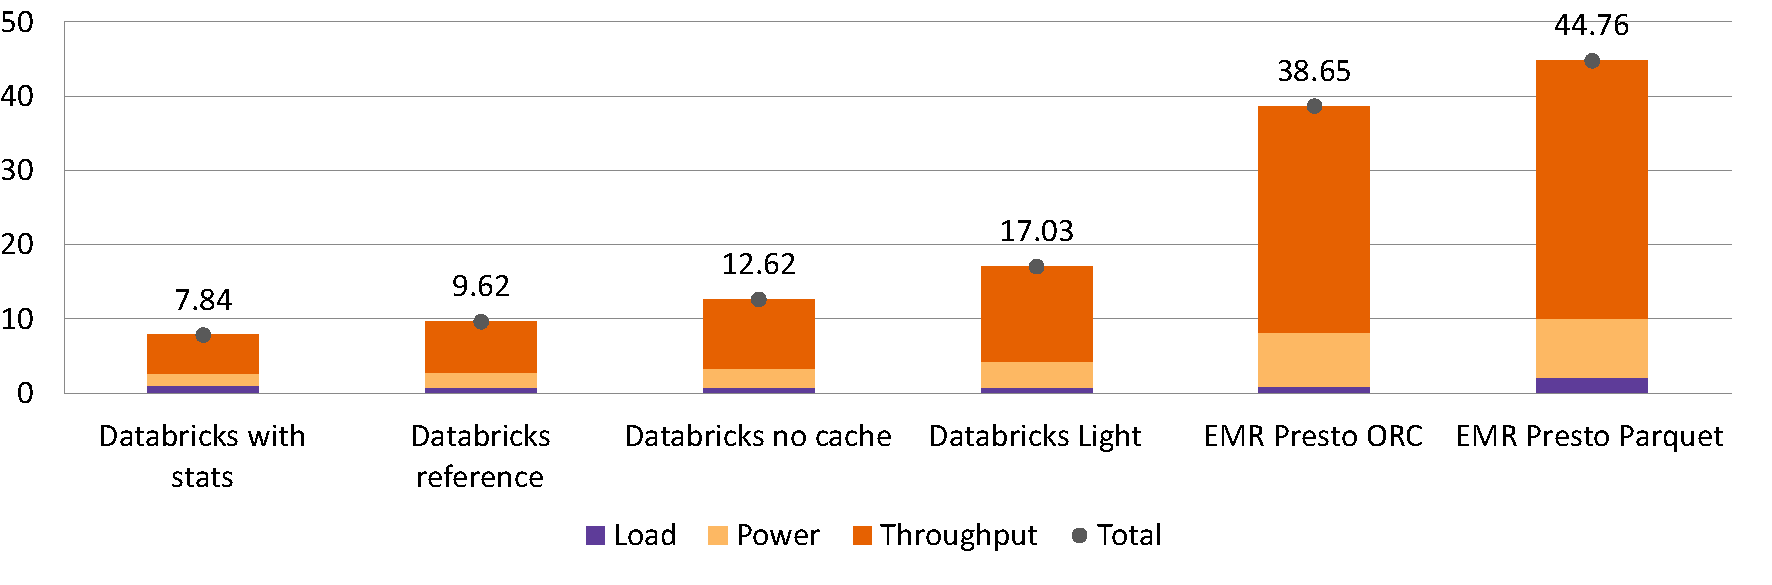
\includegraphics[width=7.0in]{imgs/resultsSummary/TotalTimes.pdf}}
   \end{center}
   \caption{TPC-DS Benchmark total execution time for various configurations.}
   \label{fig:resultsSummaryTotalTimes}
\end{figure}

The lowest total time is achieved with Databricks using the cost-based optimizer with table and column statistics. It represents an almost 5 times faster alternative than the most efficient configuration for EMR Presto. In the case of Databricks Data Engineering without the cost-based optimizer, our reference configuration, the advantage drops to about 4 times faster, still very significant. Notably, Databricks Light and EMR Presto using the ORC format show very similar performance.

\subsection{Total costs}\label{resultsSummaryTotalCost}

Regarding the monetary costs incurred to obtain the total execution times listed above, we present them in Figure \ref{fig:resultsSummaryTotalCosts}.

\begin{figure}
   \begin{center}
   \scalebox{0.75}{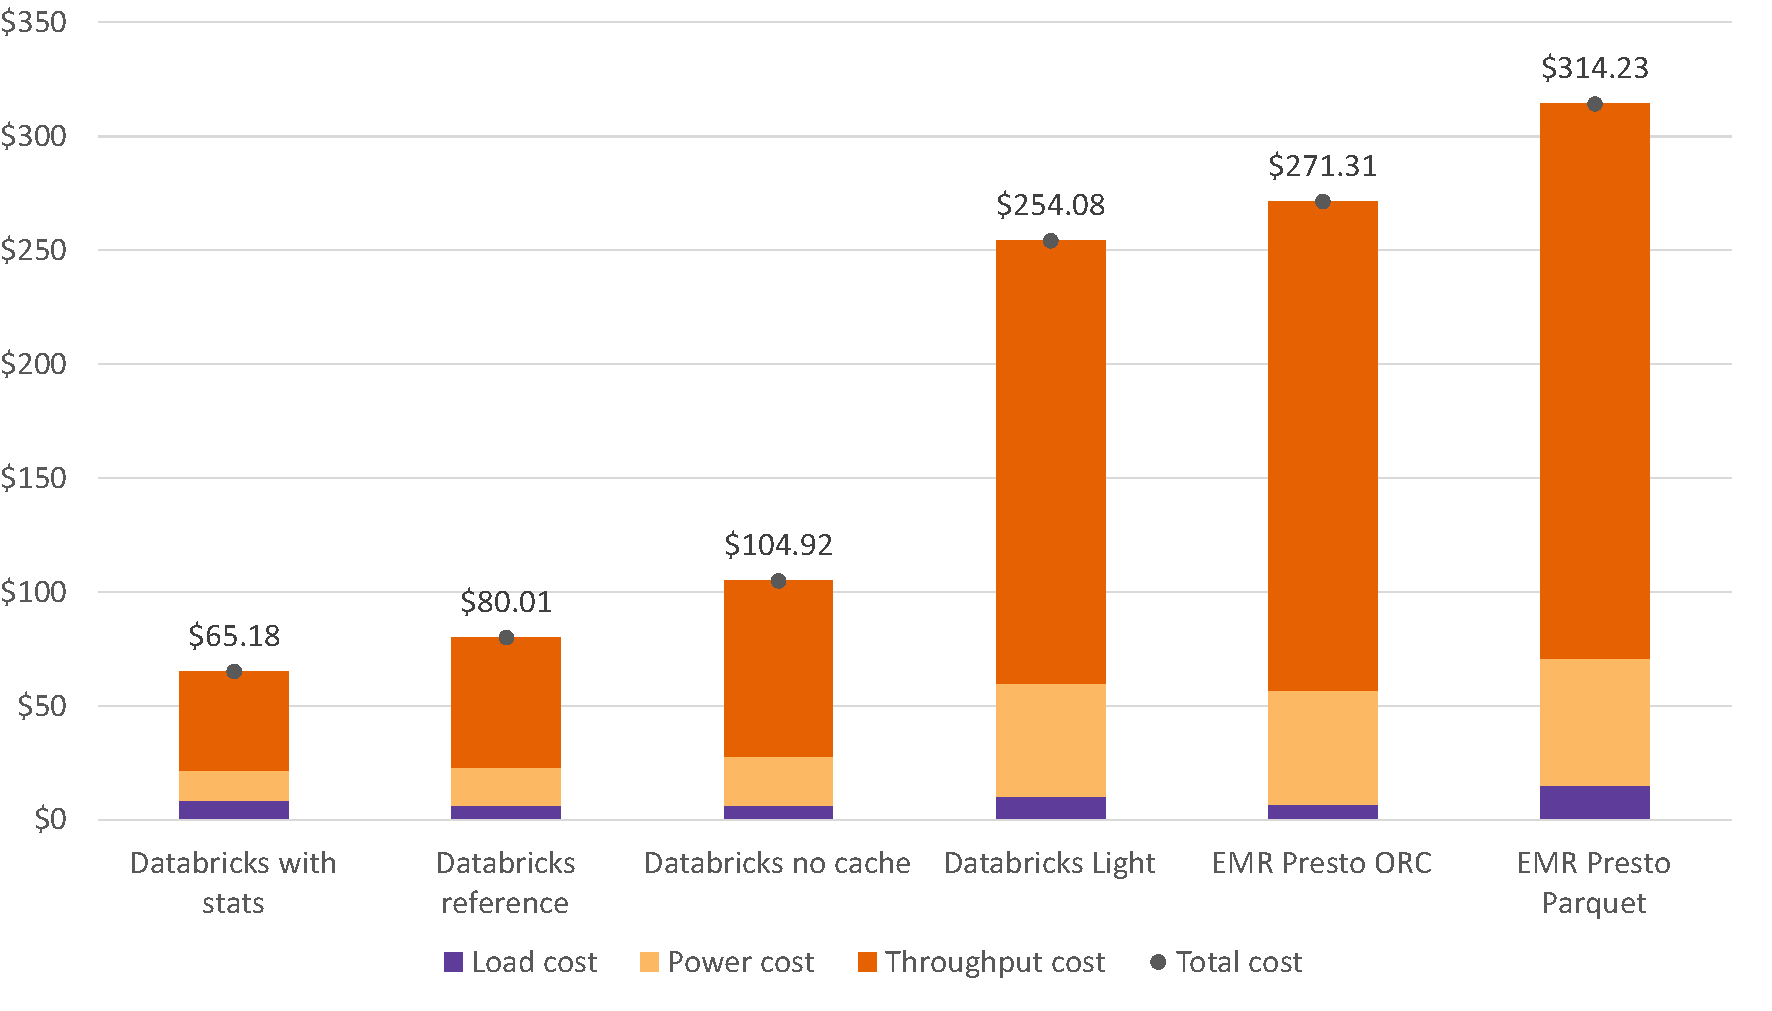
\includegraphics[width=7.0in]{imgs/resultsSummary/TotalCosts.pdf}}
   \end{center}
   \caption{TPC-DS Benchmark total execution time for various configurations.}
   \label{fig:resultsSummaryTotalCosts}
\end{figure}

\subsection{TPC-DS performance metric}\label{resultsSummaryPerformanceMetric}
